\documentclass[12pt,letterpaper]{article}
\usepackage{pdfpages}
\usepackage{fancyhdr}
\usepackage[colorlinks=true, urlcolor=blue, linkcolor=blue]{hyperref}
\usepackage{graphicx}
\usepackage[top=1.4in, left=0.5in, right=0.5in, bottom=0.8in]{geometry}
\usepackage[T1]{fontenc}
\usepackage{helvet}
\pagestyle{fancy}
\renewcommand{\headrulewidth}{0pt}
\renewcommand{\footrulewidth}{0pt}
\setlength{\parindent}{0em}
\setlength{\parskip}{1em}


\fancyfoot[C]{\setlength{\unitlength}{1in}\begin{picture}(5,0)\put(-1.8,-1){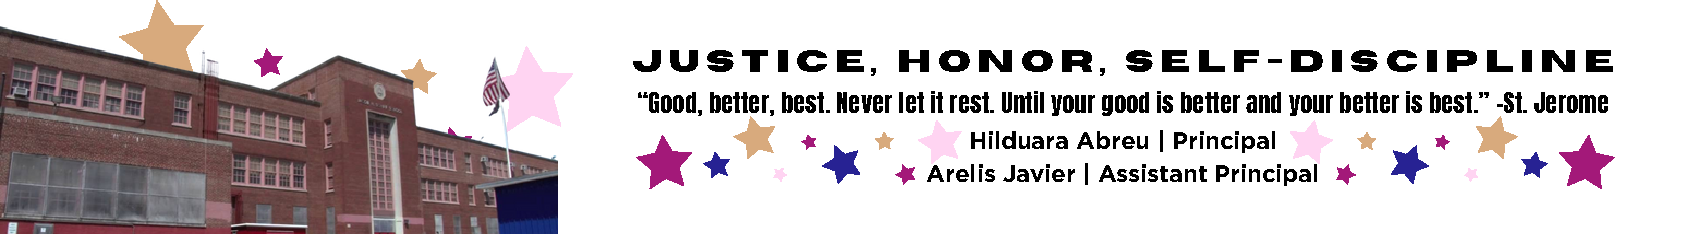
\includegraphics[width=8.8in,height=1.3in]{logo-1}}\end{picture}}
\fancyhead[C]{\setlength{\unitlength}{1in}\begin{picture}(5,0)\put(-1.9,-1){
\includegraphics[width=8.9in,height=1.3in]{logo-2}}\end{picture}}

\pagenumbering{gobble}
\addtolength{\evensidemargin}{-2in}
\addtolength{\topmargin}{-0.5in}
\addtolength{\textwidth}{0in}
%%%%%%%%%%%%%%%%%%%%%%%%%%%%%%%%%%%%%%%%%%%%%%%%%%%%%%%%%%%%%%%%%%

\begin{document}
\vspace*{0.5in}
School Website: \href{https://www.ps192.org/apps/pages/index.jsp?uREC_ID=1504973&type=d&pREC_ID=2359028}{www.ps192.org}

\textbf{Principal's Message January 2024}

Dear Esteemed Parents and Guardians,

Warmest greetings for the New Year! May this season bring health and serenity to your families. I am grateful for the collaborative spirit that has been fostered between our school and your homes, and I deeply appreciate your continued engagement in your child's educational journey.

As we embrace the fresh start that the New Year offers, it presents a wonderful chance for both you and your children to establish beneficial habits that will enhance your lives. It is also a time for introspection and to identify areas where we can all strive for growth.

At P.S. 192, a plethora of activities and events are on the horizon, each offering enriching experiences for you and your children to partake in and learn from.

Please mark your calendars for the upcoming Parent Association Meeting on January 9th at 8:00 a.m. in the Library, the Virtual SLT meeting on January 17th from 2:30 p.m. to 5:30 p.m., and Coffee with the Principal on January 24th at 8:00 a.m., also in the library.

I eagerly anticipate your participation in our events this month and look forward to the opportunity to connect with you.

Warm regards,


\includegraphics[width=0.2\textwidth]{hil_signature}

\textbf{Hilduara Abreu}

\textbf{Principal P.S. 192}

\textit{The School of Joyful Learning!}

\newpage
\vspace*{.5in}
Nuestro Sitio Web: \href{https://www.ps192.org/apps/pages/index.jsp?uREC_ID=1504973&type=d&pREC_ID=2359028}{www.ps192.org}

\textbf{Mensaje de La Directora Para Enero 2024}

Estimados padres y tutores,

¡Saludos más cordiales para el Año Nuevo! Que esta temporada traiga salud y serenidad a vuestras familias. Estoy agradecido por el espíritu de colaboración que se ha fomentado entre nuestra escuela y sus hogares, y aprecio profundamente su participación continua en el viaje educativo de su hijo.

Al acoger el nuevo comienzo que ofrece el Año Nuevo, se presenta una oportunidad maravillosa para que tanto usted como sus hijos establezcan hábitos beneficiosos que mejorarán sus vidas. También es un momento para la introspección y para identificar áreas en las que todos podemos esforzarnos por crecer.

En P.D. 192, hay una gran cantidad de actividades y eventos en el horizonte, cada uno de los cuales ofrece experiencias enriquecedoras para que usted y sus hijos participen y aprendan.

Marque en sus calendarios la próxima reunión de la Asociación de Padres el 9 de enero a las 8:00 a. m. en la biblioteca, la reunión virtual del SLT el 17 de enero a las 2:30 p. m. a 5:30 p.m., y Café con el Director el 24 de enero a las 8:00 a.m., también en la biblioteca.

Anticipo ansiosamente su participación en nuestros eventos de este mes y espero tener la oportunidad de conectarme con usted.

Un cordial saludo,


\includegraphics[width=0.2\textwidth]{hil_signature}

\textbf{Hilduara Abreu}

\textbf{Principal P.S. 192}

\textit{The School of Joyful Learning!}
\end{document}
